\documentclass[10pt,a4paper]{article}
\usepackage[utf8]{inputenc}
\usepackage{amsmath}
\usepackage{amsfonts}
\usepackage{amssymb}
\usepackage{graphicx}
\graphicspath{ {../img/} }
\author{Gradey Cullins}
\title{Assignment 2}
\begin{document}
\maketitle

\section*{3}
\textbf{Newton-cotes}\\
Constant interpolant:  6.3047    6.3051    6.3052    6.3052    6.3052    6.3052 \\
Linear interpolant:  6.3047    6.3051    6.3052    6.3052    6.3052    6.3052 \\
Quadratic interpolant: 6.3669    6.3369    6.3213    6.3133    6.3092    6.3072 \\

\noindent
\textbf{Guassian methods}\\
$N = 1 \rightarrow 6.2832 $  \\
$N = 2 \rightarrow 6.1198 $ \\
$N = 3 \rightarrow 6.3010 $ \\ 
$N = 4 \rightarrow 5.1585 $ \\
$N = 5 \rightarrow 6.6448 $  \\

% Simp:  O(dx^4)
% Mid: O(dx^2)
% Trap: O(dx^2)

\noindent
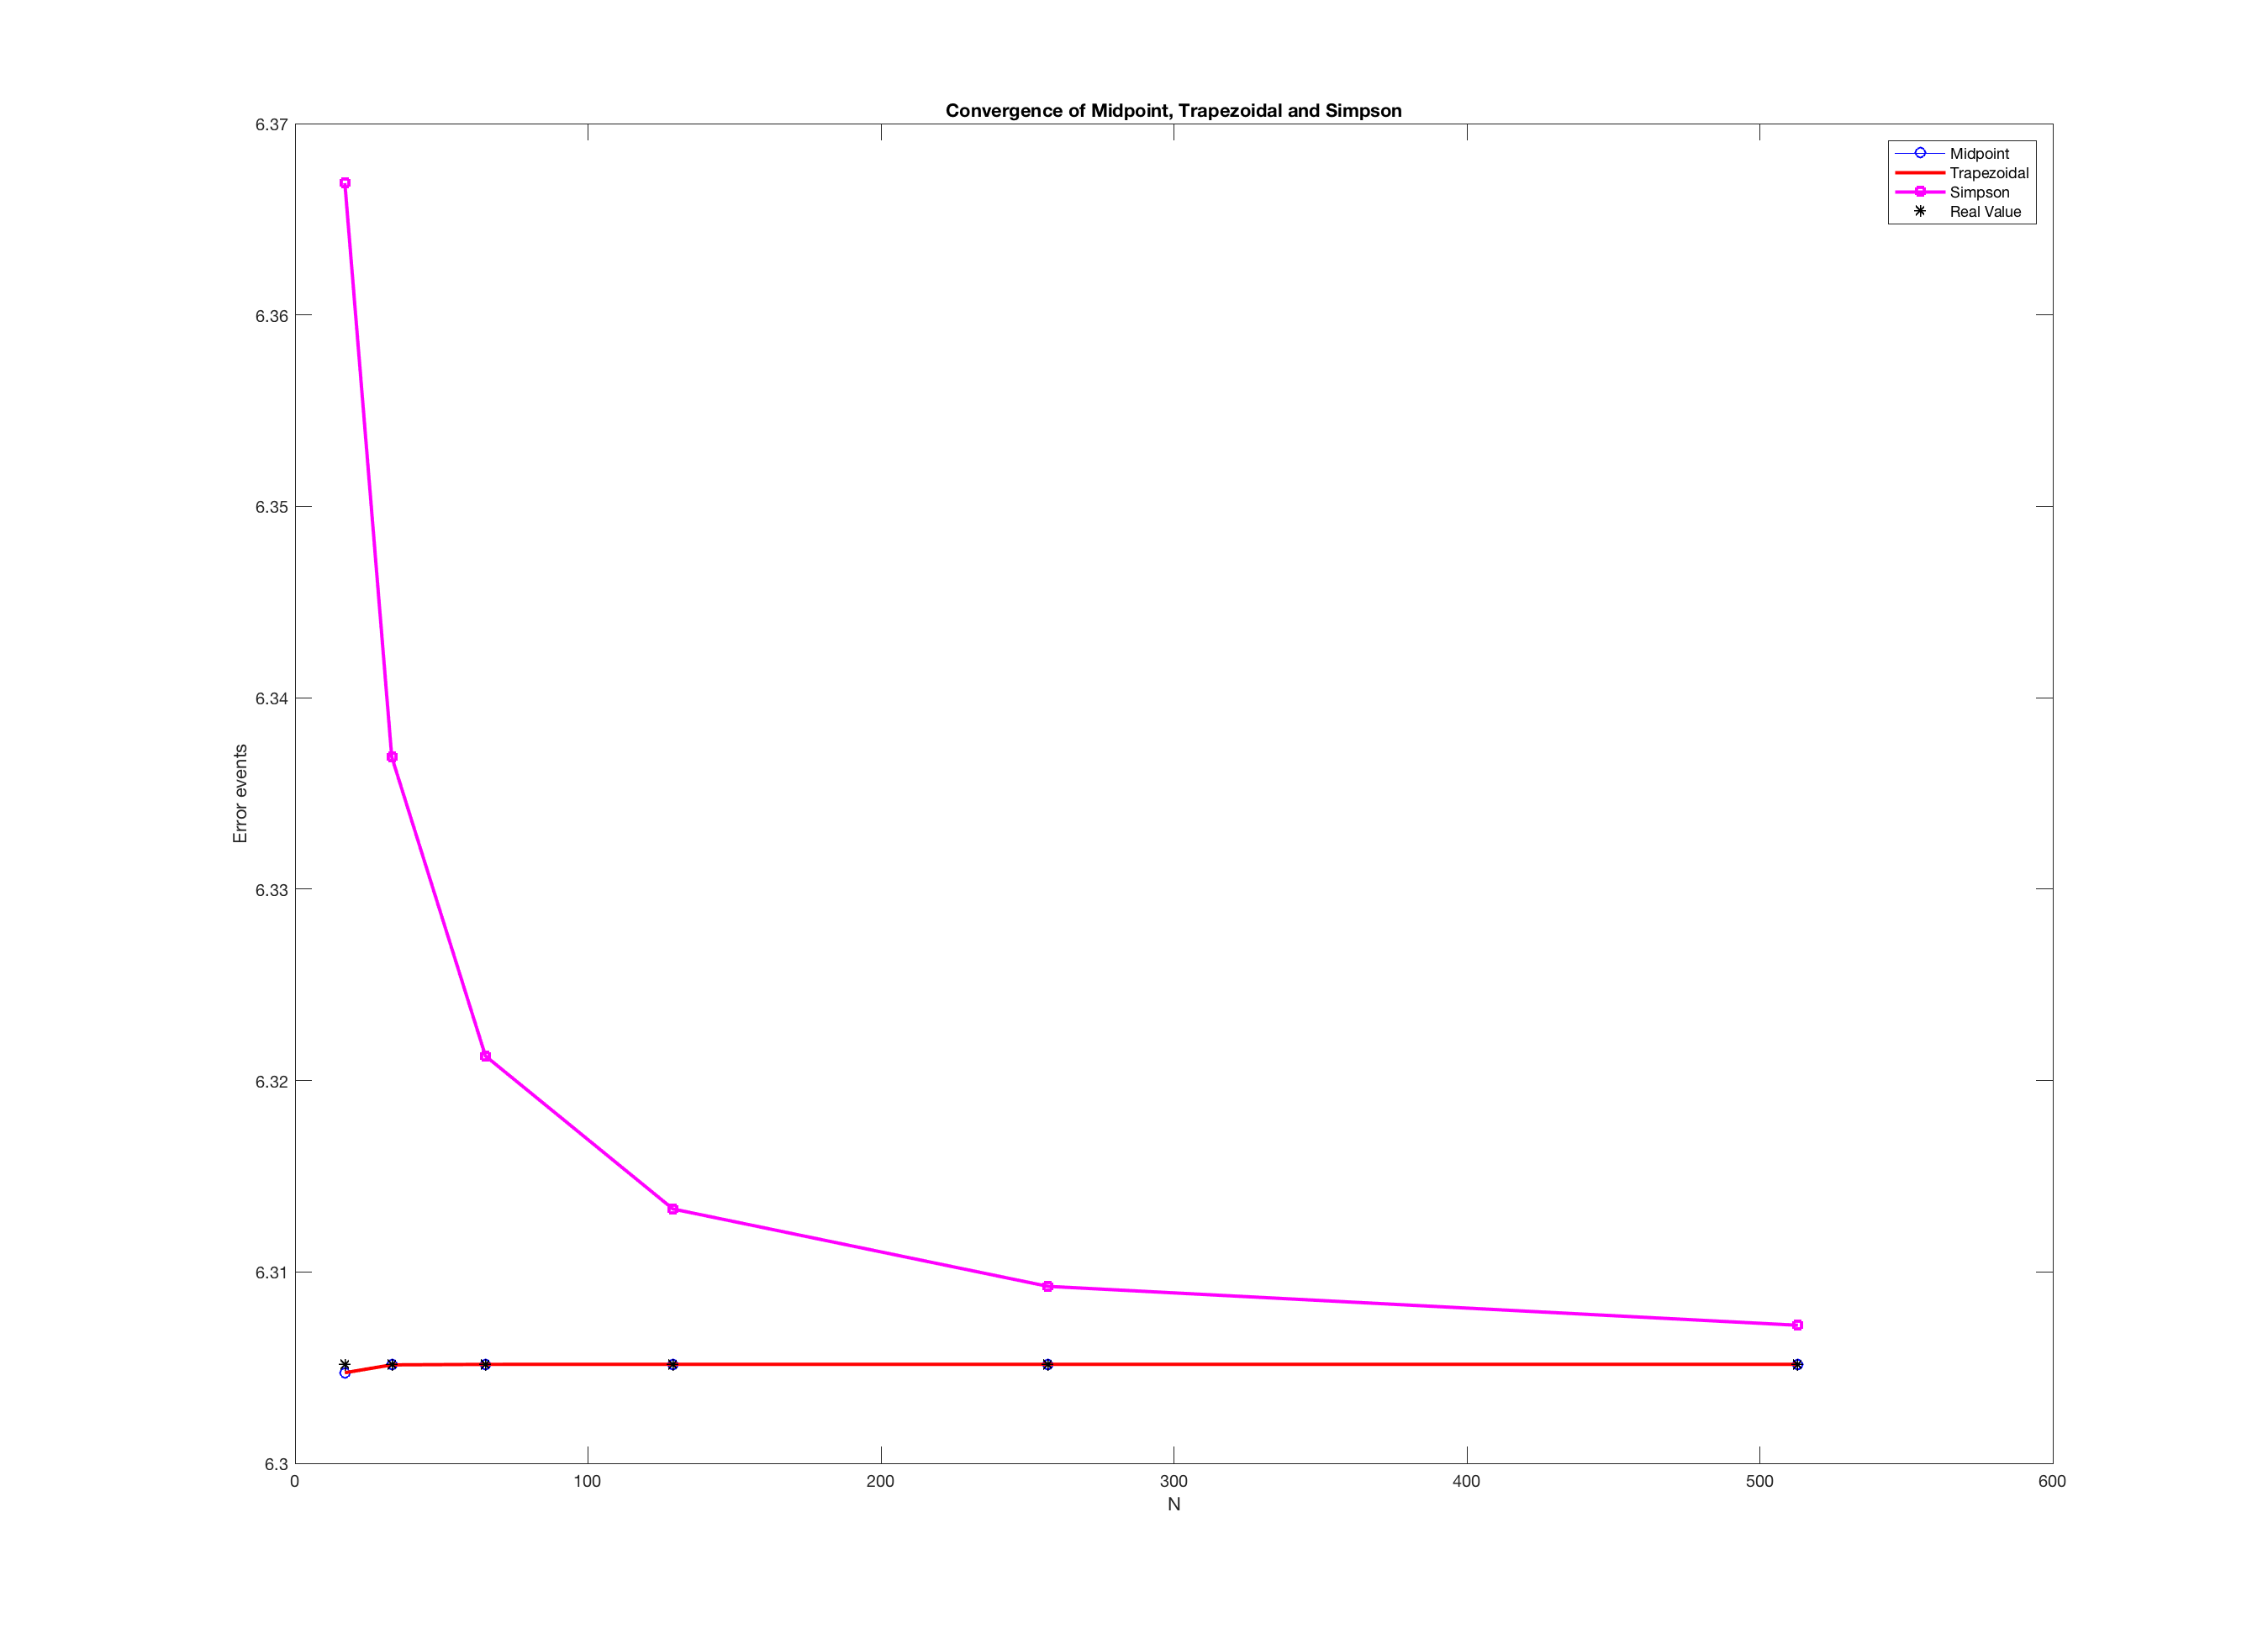
\includegraphics[scale=0.14]{cotes_convergence.png}

Trapezoidal and Midpoint converge the fastest. They also seem to converge with identical values at each step size N. This seems suspicious to me, and I have some
worry that it indicates a programmatic error on my part. The convergence of these two is much different from that of Simpson's. I believe this is in line with the
theoretical error seeing as the error of Trapezoidal and Midpoint is bound by $ O(dx^2) $, while Simpson's is bound by $ O(dx^4) $. \\

The explicit error for the Trapezoidal Rule is given by: \\ 

$ E(trap) = \frac{(b - a)dx^2 f''(\epsilon)}{12}  \rightarrow  $  1.1753, 0.3119, 0.0804,    0.0204,    0.0051,    0.0013 \\

The explicit error for the Simpson Rule is given by: \\

$ E(simp) = \frac{(b - a)dx^4 f''''(\epsilon)}{2880} $ \\ 

9.8118e-04 \\ 

6.9101e-05 \\ 

4.5908e-06 \\

2.9593e-07\\ 

1.8785e-08\\ 

1.1832e-09 \\

\noindent
The Richardson error for Trapezoidal is given by: \\
$ (\frac{4}{3}) * ( - I(trap, h) + I(trap, \frac{h}{2})) $ \\

-5.4815e-04 \\

-3.3210e-05 \\

-2.1248e-06 \\

-1.3572e-07 \\

-8.5974e-09 \\

0 \\

\noindent
The Richardson error for Simpson is given by: \\
$ (\frac{4}{3}) * ( - I(trap, h) + I(trap, \frac{h}{2})) $ \\

0.0400 \\

0.0208 \\

0.0107 \\

0.0054 \\

0.0027 \\

0 \\

\noindent
The explicit error calculations should be more accurate because they involve knowing what the function f is and require maximizing the derivatives of this function. \\

\noindent
The results for the Gaussian quadratures are reported at the beginning of this document. \\

\noindent
One explanation for why the quadratures perform poorly is that high order functions can tend to have an over-fitting effect. This often results in oscillation around the true value when the polynomial power becomes too large. Also, it is possible that the true function f is not well approximated by a polynomial in the range -1 to 1. Also, if the function f has singularities, the performance becomes even worse still. \\

\noindent
One way to improve the quadratures is to re-evalute which points are used through usage of a nested quadrature rule. Here, points can be re-chosen based on information produced by less accurate runs, thu s optimizing the polynomial fitting and reducing the error. (I sourced https://en.wikipedia.org/wiki/Gauss-Kronrod\_quadrature\_formula for this question).




\end{document}
